\documentclass{article}

%%---------------------------------------------------------------------------%%
%%	Paquetes
%%---------------------------------------------------------------------------%%
\usepackage{amsmath, amsthm}
\usepackage[spanish,activeacute]{babel}
\usepackage{wrapfig}
%\usepackage{a4wide}
\usepackage[paper=a4paper, left=3cm, right=3cm, top=4.5cm, bottom=3cm, includefoot, centering]{geometry}
\usepackage{needspace}
\usepackage{hyperref}
\usepackage[center]{caption}
\usepackage{fancyhdr}
\usepackage{graphicx}
\usepackage{capt-of}
\usepackage{lastpage}
\usepackage{afterpage}
\usepackage{float}
\usepackage{amssymb}
\usepackage{amsmath}
\usepackage[utf8]{inputenc}
\usepackage{algorithm}
\usepackage{algorithmic}
\usepackage{subfig}
\usepackage[dvipsnames,usenames]{color}
\usepackage{amsfonts}
\usepackage{amsthm}
\usepackage{pdfpages}
\usepackage[subfigure]{tocloft}
\usepackage{listings}
\usepackage{xcolor}

\colorlet{punct}{red!60!black}
\definecolor{background}{HTML}{FFFFFF}
\definecolor{delim}{RGB}{20,105,176}
\colorlet{numb}{magenta!60!black}

\lstdefinelanguage{json}{
    basicstyle=\normalfont\ttfamily,
    numbers=left,
    numberstyle=\scriptsize,
    stepnumber=1,
    numbersep=8pt,
    showstringspaces=false,
    breaklines=true,
    frame=lines,
    backgroundcolor=\color{background},
    literate=
     *{0}{{{\color{numb}0}}}{1}
      {1}{{{\color{numb}1}}}{1}
      {2}{{{\color{numb}2}}}{1}
      {3}{{{\color{numb}3}}}{1}
      {4}{{{\color{numb}4}}}{1}
      {5}{{{\color{numb}5}}}{1}
      {6}{{{\color{numb}6}}}{1}
      {7}{{{\color{numb}7}}}{1}
      {8}{{{\color{numb}8}}}{1}
      {9}{{{\color{numb}9}}}{1}
      {:}{{{\color{punct}{:}}}}{1}
      {,}{{{\color{punct}{,}}}}{1}
      {\{}{{{\color{delim}{\{}}}}{1}
      {\}}{{{\color{delim}{\}}}}}{1}
      {[}{{{\color{delim}{[}}}}{1}
      {]}{{{\color{delim}{]}}}}{1},
}
%%---------------------------------------------------------------------------%%
%%	Opciones
%%---------------------------------------------------------------------------%%

\parskip    = 11 pt
\headheight	= 13.1pt
\pagestyle	{fancy}
\definecolor{orange}{rgb}{1,0.5,0}
%\addtolength{\textheight}{-1.5cm}

%%---------------------------------------------------------------------------%%
%%	Document
%%---------------------------------------------------------------------------%%
\begin{document}
\renewcommand{\partname}{Capítulo}
\renewcommand{\tablename}{Tabla}
\renewcommand{\algorithmicrequire}{\textcolor{blue}{\textbf{Requiere:}}}
\renewcommand{\algorithmicensure}{\textbf{Asegura:}}
\renewcommand{\algorithmicend}{\textbf{Fin}}
\renewcommand{\algorithmicif}{\textcolor{blue}{\textbf{Si}}}
\renewcommand{\algorithmicthen}{\textcolor{blue}{\textbf{entonces}}}
\renewcommand{\algorithmicelse}{\textcolor{red}{\textbf{Si no}}}
\renewcommand{\algorithmicelsif }{\textcolor{blue}{\textbf{Si no y}}}
\renewcommand{\algorithmicendif}{\textcolor{blue}{\textbf{Fin si}}}
\renewcommand{\algorithmicfor}{\textcolor{ForestGreen}{\textbf{Para}}}
\renewcommand{\algorithmicendfor}{\textcolor{ForestGreen}{\textbf{Fin para}}}
\renewcommand{\algorithmicwhile}{\textcolor{ForestGreen}{\textbf{Mientras}}}
\renewcommand{\algorithmicendwhile}{\textcolor{ForestGreen}{\textbf{Fin mientras}}}
\renewcommand{\algorithmicdo}{\textcolor{ForestGreen}{\textbf{hacer}}}
\renewcommand{\algorithmicreturn}{\textbf{Devolver}}
\floatname{algorithm}{Algoritmo}


\newcommand{\referencia}[1]{(ver ~\ref{#1})}
%% Redefine the \paragraph command: 
\makeatletter 
\renewcommand\paragraph{\@startsection{paragraph}{4}{0mm}% 
{-\baselineskip}% 
{0.5\baselineskip}% 
{\normalfont\bfseries}% 
}%
\@addtoreset{figure}{part}
\@addtoreset{table}{part}
\@addtoreset{algorithm}{part}
\@addtoreset{section}{part}
\makeatother
\cftsetindents{section}{1em}{2em}
\cftsetindents{subsection}{2em}{3em}
\cftsetindents{subsubsection}{3em}{4em}
\setlength{\cftparskip}{0.2em}

%%---------------------------------------------------------------------------%%
%% Caratula
%%---------------------------------------------------------------------------%%

\includepdf{caratula.pdf}

% Pagina en blanco para imprimir doble faz
\newpage
\thispagestyle{empty}
\mbox{}

\pagestyle{empty}{
\begin{abstract}
La arquitectura Q fue creada en la Universidad Nacional de Quilmes con el propósito de facilitar la enseñanza y el aprendizaje de lenguajes de bajo nivel, 
como assembler, en la materia Organización de Computadoras. Esta es una arquitectura conceptual, es decir, no existe una máquina física que funcione sobre dicha arquitectura.
Al ser Organización de Computadoras una materia inicial, los estudiantes encuentran una dificultad en el aprendizaje, marcado principalmente por la poca abstracción con la que cuentan estos lenguajes, sumando en nuestro caso, la imposibilidad de ejecutar sus programas. En este sentido, QSim, un trabajo de inserción 
profesional presentado en la misma universidad, aborda el problema brindando un entorno de ejecución para el lenguaje Q. Dicho proyecto fue encarado con 
una aplicación de escritorio escrita en Java que permitía ver los componentes de la arquitectura Q en funcionamiento. Algunos de los problemas que se 
encontraron a esta implementación fueron la baja performance de la herramienta y la dificultad que encuentran los estudiantes para configurar el entorno
 que requiere la aplicación para funcionar. 
 
Es por eso que en este trabajo se busca brindar una solución a este problema: un simulador de la arquitectura Q que permita visualizar de manera didáctica el proceso de 
ejecución de un lenguaje de bajo nivel pero realizada en un entorno web, lo cual evita las complejidades accidentales encontradas y nombradas 
anteriormente y agrega portabilidad para diversos dispositivos como celulares o tablets. Además, en contexto de la Pandemia por COVID-19, donde la 
educación en la Universidad tuvo un viraje a la educación virtual, es fundamental contar con una herramienta que pueda ser accedida mediante Internet.
El trabajo brinda una librería escrita en javascript que implementa el lenguaje Q y una interfaz visual que utiliza esa librería para mostrar de manera
 didáctica el proceso de ejecución. Esta separación permite realizar cambios en la interfaz de usuario sin afectar a la lógica del lenguaje.
\end{abstract}

\renewcommand{\abstractname}{Abstract}
\begin{abstract}
The Q architecture was created at the Universidad Nacional de Quilmes with the purpose of helping to teach and learn low-level languages, such as Assembly, in the context of the course of study Computer Organization.
It's a conceptual architecture, meaning that there is not a physical computer that works with it. 
Students often face a learning difficulty caused mainly by the lack of abstraction that these languages have, adding in our case the fact that Computer Organization is an initial subject and the impossibility of executing their programs.
Given this, QSim, a TIP presented at the same university, addresses the problem by providing an execution environment for the Q language.
The project was developed as a Java desktop application, which made it resource hungry and hard to set up.

Therefore this project tries to provide a solution to this problem: 
a tool that allows to didactically visualize the process of executing a low-level language while running on a web environment, 
which avoids the accidental complexities found in QSim and that also adds portability for various devices such as cell phones or tablets.
Moreover, in the context of a pandemic due to COVID-19, and universities embracing virtual learning, an online tool becomes even more significant.
This project provides a library written in javascript that implements the Q language and a visual interface that uses said library to display the execution process in a more didactic way. 
This separation allows changes to be made to the user interface without altering the language’s logic.
\end{abstract}

}

\pagestyle{empty}
{
\fancypagestyle{plain}
    {
    \fancyhead{}
    \fancyfoot{}
    \renewcommand{\headrulewidth}{0.0pt}
    } % clear header and footer of plain page because of ToC
%\setcounter{tocdepth}{5}
%\setcounter{secnumdepth}{5}


% Pagina en blanco para imprimir doble faz
\newpage
\thispagestyle{empty}
\mbox{}
\newpage
\thispagestyle{empty}
\mbox{}



\tableofcontents
}

% Arregla los estilos para el resto del documento, y
% resetea los numeros de pagina para que queden bien.
\newpage
\pagenumbering{arabic}
\fancypagestyle{plain} {
    \fancyhead[LO]{Perez, Pissi--Martinez}
    \fancyhead[C]{}
    \fancyhead[RO]{P\'agina \thepage\ de \pageref{LastPage}}
    \fancyfoot{}
    \renewcommand{\headrulewidth}{0.4pt}
}
\pagestyle{plain}

\newenvironment{packed_itemize}{
\vspace{-0.5cm}
\begin{itemize}
\setlength{\itemsep}{1pt}
\setlength{\parskip}{0pt}
\setlength{\parsep}{0pt}
}{\end{itemize}}

\renewcommand{\thepart}{\arabic{part}}
\renewcommand{\thefigure}{\arabic{part}.\arabic{figure}}
\renewcommand{\thetable}{\arabic{part}.\arabic{table}}
\renewcommand{\thealgorithm}{\arabic{part}.\arabic{algorithm}}
\renewcommand{\thesection}{\arabic{part}.\arabic{section}}

\part*{Agradecimientos}
\begin{itemize}
  \item A Federico Martinez por sus grandes aportes conceptuales, por su buena onda y predisposición para ayudar.
  \item Al equipo docente de Organización de Computadoras por brindarnos su perspectiva y apoyo sobre el diseño de la herramienta. 
\end{itemize}

\section*{Agradecimientos de Francisco}
\begin{itemize}
  \item A Pablo, por confiar en mí y ofrecerme trabajar con él en este hermoso proyecto.
  \item A Fede, por acompañarnos siempre, aguantarnos y compartir de su humor y sabiduría.
  \item A mis compañeros, amigos y familia, por siempre estar ahí apoyándome y escuchándome.
  \item A la Universidad Nacional de Quilmes, por el maravilloso clima que siempre genera, haciendo que sin importar quien esté en ella, se sienta cómodo y bienvenido.
\end{itemize}

\section*{Agradecimientos de Pablo}
\begin{itemize}
  \item A Fede por invitarme a colaborar con la materia y darme libertad para crecer en la docencia.
  \item A Tati por escucharme hablar de mis cursadas como si fuese algo novedoso para ella.
  \item A la dirección de la carrera, en especial Gabi, que siempre estuvo para darme una mano.
  \item A mis compañeros y compañeras, que me ayudaron a llegar hasta dónde estoy, muchas veces en sentido literal.
  \item A mi familia y amigos por escuchar mis explicaciones con más amor que entendimiento.
\end{itemize}

\part{Introducción}
\label{introduccion}

La materia Organización de Computadoras es dictada en el ciclo básico de la Tecnicatura Universitaria en Programación Informática de la Universidad Nacional 
de Quilmes y brinda contenidos que aportan un panorama general sobre arquitectura de computadoras. 
Nuestras computadoras utilizan una arquitectura llamada Arquitectura de Von Neumann, la cual consta de una Unidad Central de Procesamiento (CPU por sus 
siglas en inglés) y una memoria donde se almacenarán tanto los datos como los programas. Para interactuar con la arquitectura se utilizan lenguajes de 
programación de bajo nivel, como puede ser el lenguaje ensamblador.
Una de las implementaciones de la Arquitectura de Von Neumann es x86, la arquitectura creada por Intel que sirve como modelo para los procesadores actuales.

Para poder ejecutar un programa este debe ser ensamblado en memoria. El ensamblado consiste en convertir el código de lenguaje ensamblador en código 
binario.
El proceso de ejecución en la arquitectura de Von Neumann consta de 3 etapas: fetch, decode, execute.
La etapa fetch se encarga de buscar las instrucciones previamente ensambladas en memoria.
Una vez que se encontraron las instrucciones en memoria, estas son decodificadas en la etapa de decode, donde se resuelven los valores de sus operandos, si
hubiese alguno.
Como paso final, se ejecuta la instrucción en la etapa de execute. Dicha ejecución puede llevar a cabo cambios en el estado de la computadora.

En la materia Organización de Computadoras se creó una arquitectura conceptual llamada Q, utilizando el modelo de la Arquitectura de Von Neumann. Dicha arquitectura se define como conceptual ya que no existe una máquina física que funcione en ella.
A su vez, esta arquitectura cuenta con el lenguaje homónimo para su utilización. Está pensada para la enseñanza de arquitecturas de computadoras en un nivel inicial.

Como la materia es dictada en el ciclo básico, muchos/as estudiantes encuentran la complejidad de no poder ver el resultado de sus programas, ya que deben comprender los conceptos para poder simularlos manualmente. En este sentido, QSim, un simulador de la arquitectura Q que fue desarrolado hace algunos años en el contexto de otro trabajo de inserción profesional realiza un aporte significativo, brindando una interfaz visual para la ejecución de programas Q. Sin embargo, dadas las tecnologías y el paradigma de diseño de aplicaciones utilizado, resulta dificultoso para los y las estudiantes su uso actual. Algunos de los inconvenientes encontrados son:
\begin{itemize}
\item Quienes quieren usarlo, deben tener instalado un conjunto de aplicaciones, lo cual aporta complejidades accidentales que podrían ser evitadas.
\item No puede ser utilizado en dispositivos móviles, ya que las tecnologías utilizadas y la solución propuesta no contemplaban el uso masivo de dispositivos móviles que vemos actualmente.
\item Falta de accesibilidad para personas que utilicen lectores de pantalla.
\item Tiene problemas de rendimiento, como la baja velocidad.
\end{itemize}

Es por eso que se decidió realizar una implementación del lenguaje Q utilizando las tecnologías y paradigmas actuales, evitando las dificultades encontradas en las herramientas mencionadas. El propósito de este trabajo es crear un simulador que permita ejecutar programas en la arquitectura Q. De esta manera las y los estudiantes de la materia tendrán la posibilidad de escribir programas en dicho lenguaje y ver el impacto de los mismos en las partes que componen a la arquitectura, como son registros, memoria, flags y registros especiales. Esta herramienta debe cumplir las siguientes propiedades:

\begin{itemize}
\item Poder ejecutar cualquier programa de la arquitectura Q.
\item Permitir la visualización de los resultados o los errores de ejecución.
\item No requerir instalación.
\item Poder usarse desde dispositivos móviles.
\item Ser accesible para estudiantes con disminución visual o daltonismo.
\end{itemize}

A su vez, este trabajo tiene como objetivo la creación de una librería escrita en javascript, que pueda ser utilizada por otras herramientas que busquen un objetivo similar, separando la lógica del lenguaje de su visualización, permitiendo así, mantener actualizadas las herramientas visuales sin tener que actualizar la lógica del lenguaje.


\section{Resumen del trabajo}

\label{resumen}

Esta trabajo se organiza de la siguiente manera:

\begin{itemize}
\item El capítulo \ref{introduccion} es esta introducción, que pretende establecer el concepto de Arquitectura de computadoras de manera básica,
la arquitectura Q planteada en la universidad y las motivaciones que llevan al desarrollo de QSim Web, incluyendo un análisis de las herramientas existentes.

\item El capítulo \ref{arquitectura-q} explicará más en detalle la estructura de la arquitectura Q, definiendo sus capas y los conceptos
que se introducen en cada una de ellas.

\item El capítulo \ref{qsimweb} realiza una descripción de la totalidad del trabajo, diferenciando la interfaz de usuario de la librería QLib.
\item El capítulo \ref{devoluciones} cuenta las devoluciones de los y las estudiantes luego de haber utilziado la herramienta durante un cuatrimestre.
\item El capítulo \ref{parte_conclusiones} describe las conclusiones desarrolladas a partir de la realización del trabajo.

\end{itemize}

\part{Arquitectura Q}
\label{arquitectura-q}
En la materia Organización de Computadoras se creó una arquitectura de computadoras teórica llamada Q, utilizando el modelo de la Arquitectura de Von Neumann. 
A su vez, esta arquitectura cuenta con el lenguaje homónimo para su utilización. Está pensada para la enseñanza de conceptos de organización y arquitecturas de computadoras
en un nivel inicial.

Su diseño está dividido en 5 capas llamadas Q1, Q2, Q3, Q4, Q5. Cada capa contiene a las instrucciones y modos de direccionamiento
de la capa anterior, agregando nuevas funciones a la misma. Esto permite que un programa escrito en Q1 pueda ser ejecutado en Q5, obteniendo el mismo resultado.

\section{Q1}
El objetivo de esta capa es introducir algunos conceptos básicos de la programación de lenguajes de bajo nivel, como son las instrucciones, registros e inmediatos.

Sus caracteristicas son: 8 registros de uso general, llamados desde R0 a R7; un modo de direccionamiento para trabajar con constantes llamado Inmediato y 5 instrucciones de dos operandos cada una, MOV, ADD, SUB, DIV, MUL.

Los registros tienen 16 bits de almacenamiento. Los inmediatos tienen 16 bits de longitud y se escriben en hexadecimal con la 
sintaxis: 0xAAAA.

Las instrucciones de esta capa son:
\begin{table}[H]
  \label{tab:instrucciones}
  \begin{center}
    \begin{tabular}{| c | c | c | c |}
      \hline
      \textbf{Operación} & \textbf{Cod Op} & \textbf{Efecto}                                   & \textbf{Ejemplo de uso}   \\ \hline
      ADD                & 0010            & destino \leftarrow destino + origen               & ADD R7, 0x23FA            \\ \hline
      DIV                & 0111            & destino \leftarrow destino \% origen              & DIV R4, 0x23FA            \\ \hline
      MOV                & 0001            & destino \leftarrow origen                         & MOV R4, R2                \\ \hline
      MUL                & 0000            & destino \leftarrow destino \times origen          & MUL R5, 0x0ABC            \\ \hline
      SUB                & 0011            & destino \leftarrow destino - origen               & SUB R2, [0x0ABC]          \\ \hline
    \end{tabular}
  \end{center}
\end{table}
Todas estas instrucciones comparten el siguiente formato:
\begin{table}[H]
  \label{tab:formatoinstruccion}
  \begin{center}
    \begin{tabular}{| c | c | c | c | c |}
      \hline
      \textbf{Cod Op} & \textbf{Modo Destino} & \textbf{Modo Origen} & \textbf{Destino} & \textbf{Origen} \\ \hline
      4 bits          & 6 bits                & 6 bits               & 16 bits          & 16 bits         \\ \hline
    \end{tabular}
  \end{center}
\end{table}

Los modos de direccionamiento son:
\begin{threeparttable}
  \begin{center}
    \label{tab:modosQ1}
    \begin{tabular}{| l | l |}
      \hline
      \textbf{Modo}      & \textbf{Codificación} \\ \hline
      Inmediato          & 000000                \\ \hline
      Registro           & 100rrr \footnotemark              \\ \hline
    \end{tabular}
    \footnotetext[1]{ La codificación de un registro varía según el número del mismo. R2 se codifica 100010 ya que 2 se representa como 010 en BSS(3).}
  \end{center}
\end{table}

Un ejemplo de instrucción invalida es: ADD 0x23FA, R7 porque una constante no puede almacenar el resultado de una operación.

Un ejemplo de ensamblado de la instrucción ADD R6, 0x2323 en la celda 0x00F0
\begin{table}[H]
  \label{tab:formatoinstruccion}
  \begin{center}
    \begin{tabular}{| c | c | c | c | c |}
      \hline
      \textbf{Celda}  & \textbf{Valor}               \\ \hline
      ...             & ...                          \\ \hline
      0x00F0          & 0010 100110 000000           \\ \hline
      0x00F1          & 0010 0011 0010 0011          \\ \hline
      ...             & ...                          \\ \hline
    \end{tabular}
  \end{center}
\end{table}

\section{Q2}
El objetivo de esta capa es brindar la posibilidad de interactuar con la memoria, algo que se omite en Q1 por simplicidad.

Para ello, se agrega un modo de direccionamiento llamado Directo el cual especifica la dirección de memoria donde se encuentra el valor del operando. La dirección del 
operando se escribe entre corchetes: [0x23AB].

Los modos de direccionamiento son:
\begin{threeparttable}
  \begin{center}
    \label{tab:modosQ1}
    \begin{tabular}{| l | l |}
      \hline
      \textbf{Modo}      & \textbf{Codificación} \\ \hline
      Inmediato          & 000000                \\ \hline
      Registro           & 100rrr                \\ \hline
      \textbf{Directo}   & \textbf{001000}       \\ \hline
    \end{tabular}
  \end{center}
\end{table}

Un ejemplo de ensamblado de la instrucción ADD R6, [0x2323] en la celda 0x00F0
\begin{table}[H]
  \label{tab:formatoinstruccion}
  \begin{center}
    \begin{tabular}{| c | c | c | c | c |}
      \hline
      \textbf{Celda}  & \textbf{Valor}               \\ \hline
      ...             & ...                          \\ \hline
      0x00F0          & 0010 100110 001000           \\ \hline
      0x00F1          & 0010 0011 0010 0011          \\ \hline
      ...             & ...                          \\ \hline
    \end{tabular}
  \end{center}
\end{table}


\section{Q3}
El objetivo de esta capa es brindar la posibilidad de escribir rutinas, que permiten explicar los conceptos de reutilización, modularización y documentación.

En esta capa toman relevancia los registros PC, SP, IR, MAR, MBR y los conceptos de pila y etiqueta.
\begin{itemize}
  \item El PC es un registro especial que sirve para indicar a la CPU cuál es la siguiente instrucción a ejecutar. 
  Al leer una instrucción su valor se incrementa en 1.
  \item La pila es una sección reservada de la memoria principal para almacenar las direcciones de retorno de las rutinas invocadas.
  \item El SP es un registro especial que funciona como puntero a la pila. Es utilizado por las instrucciones CALL y RET descriptas a continuación.
  \item El IR es un registro especial que contiene la instrucción que está siendo ejecutada (o parte de ella). Tiene 48 bits de almacenamiento.
  \item El MAR es un registro especial que contiene la dirección de memoria que se está leyendo o escribiendo.
  \item El MBR es un registro especial que contiene el valor de la dirección de memoria que indica el MAR.
  \item Las etiquetas son cadenas de texto que se utilizan para abstraer el valor de una constante. Se pueden utilizar como operando de la
  instrucción CALL. Sus nombres no pueden repetirse ya que funcionan como identificadores.
\end{itemize}

Además de las caracteristicas de las capas anteriores, en esta capa se agregan dos instrucciones: CALL y RET que permiten interactuar con rutinas.

CALL: Invoca a una rutina, para ello guarda el PC en la pila, decrementa el SP en 1 y copia el PC a la dirección de memoria donde está ensamblada la primera instrucción de dicha rutina. 

Su formato de instrucción es:
\begin{table}[H]
  \label{tab:formatoinstruccion}
  \begin{center}
    \begin{tabular}{| c | c | c | c |}
      \hline
      \textbf{Cod Op} & \textbf{Relleno} & \textbf{Modo Origen} & \textbf{Origen} \\ \hline
      4 bits          & 6 bits                & 6 bits          & 16 bits         \\ \hline
    \end{tabular}
  \end{center}
\end{table}

Un ejemplo de uso es:
\begin{center}
  CALL calcularPromedio
\end{center}

RET: Finaliza la ejecución de una rutina, para ello incrementa el SP y pone en el PC el valor de la pila.

Su formato de instrucción es:
\begin{table}[H]
  \label{tab:formatoinstruccion}
  \begin{center}
    \begin{tabular}{| c | c | c |}
      \hline
      \textbf{Cod Op} & \textbf{Relleno}  \\ \hline
      4 bits          & 12 bits           \\ \hline
    \end{tabular}
  \end{center}
\end{table}

Su uso es:
\begin{center}
  RET
\end{center}

Las instrucciones de esta capa son:
\begin{table}[H]
  \label{tab:instrucciones}
  \begin{center}
    \begin{tabular}{| c | c | c | c |}
      \hline
      \textbf{Operación} & \textbf{Cod Op} & \textbf{Efecto}                                                  & \textbf{Ejemplo de uso}   \\ \hline
      ADD                & 0010            & destino \leftarrow destino + origen                              & ADD R7, 0x23FA            \\ \hline
      DIV                & 0111            & destino \leftarrow destino \% origen                             & DIV R4, 0x23FA            \\ \hline
      MOV                & 0001            & destino \leftarrow origen                                        & MOV R4, R2                \\ \hline
      MUL                & 0000            & destino \leftarrow destino \times origen                         & MUL R5, 0x0ABC            \\ \hline
      SUB                & 0011            & destino \leftarrow destino - origen                              & SUB R2, [0x0ABC]          \\ \hline
      CALL               & 1011            & [SP] \leftarrow PC ; SP \leftarrow SP - 1 ; PC \leftarrow origen & CALL unaRutina            \\ \hline
      RET                & 1100            & SP \leftarrow SP + 1 ; PC \leftarrow [SP]                        & RET                       \\ \hline
    \end{tabular}
  \end{center}
\end{table}

\section{Q4}
El objetivo de esta capa es introducir los conceptos de ejecución condicional y repeticiones. Para ello se introducen los conceptos de flags y saltos.
Los flags son registros de 1 bit que se calculan al ejecutarse instrucciones aritméticas. 
\begin{itemize}
  \item Z: es 1 cuando el resultado de la operación es 0.
  \item N: es 1 cuando el resultado de la operación es negativo.
  \item C: es 1 cuando el resultado de la operación tiene carry o borrow en el bit más significativo.
  \item V: es 1 cuando el resultado de la operación tiene overflow en complemento a 2.
\end{itemize}

Las caracteristicas de esta capa son, además de las mencionadas anteriormente, saltos condicionales relativos y saltos incondicionales absolutos.

La instrucción salto incondicional absoluto es JMP, que copia el PC a la dirección de memoria indicada por su etiqueta.

Su formato de instrucción es:
\begin{table}[H]
  \label{tab:formatoinstruccion}
  \begin{center}
    \begin{tabular}{| c | c | c | c |}
      \hline
      \textbf{Cod Op} & \textbf{Relleno} & \textbf{Modo Origen} & \textbf{Origen} \\ \hline
      4 bits          & 6 bits                & 6 bits          & 16 bits         \\ \hline
    \end{tabular}
  \end{center}
\end{table}

Un ejemplo de uso es:
\begin{center}
  JMP esNumeroPositivo
\end{center}

Las instrucciones de saltos condicionales relativos son las nombradas a continuación, cuya ejecución tiene como efecto incrementar o decrementar el PC dado un desplazamiento, si su condición de salto se cumple.

\begin{table}[H]
  \begin{center}
    \begin{tabular}{| c | c | c | c | c |}
      \hline
      \textbf{Operación} & \textbf{Cod Op}         & \textbf{Descripción}    & \textbf{Condición de salto}   & \textbf{Ejemplo de uso} \\ \hline
      JE                 & 0001                    & Igual / Cero            & Z                             & JE etiqueta             \\ \hline
      JNE                & 1001                    & No igual                & not Z                         & JNE etiqueta            \\ \hline
      JLE                & 0010                    & Menor o igual           & Z or (N xor V)                & JLE etiqueta            \\ \hline
      JG                 & 1010                    & Mayor                   & not (Z or (N xor V))          & JG etiqueta             \\ \hline
      JL                 & 0011                    & Menor                   & N xor V                       & JL etiqueta             \\ \hline 
      JGE                & 1011                    & Mayor o igual           & not (N xor V)                 & JGE etiqueta            \\ \hline
      JLEU               & 0100                    & Menor o igual sin signo & C or Z                        & JLEU etiqueta           \\ \hline
      JGU                & 1100                    & Mayor sin signo         & not (C or Z)                  & JGU etiqueta            \\ \hline
      JCS                & 0101                    & Carry / Menor sin signo & C                             & JCS etiqueta            \\ \hline
      JNEG               & 0110                    & Negativo                & N                             & JNEG etiqueta           \\ \hline
      JVS                & 0111                    & Overflow                & V                             & JVS etiqueta            \\ \hline
    \end{tabular}
    \label{tab:saltos}
  \end{center}
\end{table}
Su formato de instrucción es:
\begin{table}[H]
  \label{tab:formatoinstruccion}
  \begin{center}
    \begin{tabular}{| c | c | c |}
      \hline
      \textbf{Prefijo} & \textbf{Cod Op} & \textbf{Desplazamiento} \\ \hline
      4 bits           & 4 bits           & 8 bits                 \\ \hline
    \end{tabular}
  \end{center}
\end{table}

\section{Q5}
En esta última capa se definen dos modos de direccionamiento indirectos, que permiten el trabajo con recorridos, arreglos e iteraciones. Si bien es técnicamente posible realizar lo mencionado sin estos modos, agregaría una complejidad no buscada en la materia.
Estos modos de direccionamiento son Indirecto e Indirecto Registro. 

El modo de direccionamiento Indirecto especifica la dirección de memoria donde se encuentra la dirección de memoria que contiene el valor del operando. La dirección del 
  operando se escribe entre doble corchetes: [[0x23AB]].

El modo de direccionamiento Indirecto Registro especifica el registro donde se encuentra la dirección de memoria que contiene el valor del operando. El registro se escribe entre corchetes: [R5].

Los modos de direccionamiento y sus codificiones son:
\begin{threeparttable}
  \begin{center}
    \label{tab:modosQ1}
    \begin{tabular}{| l | l |}
      \hline
      \textbf{Modo}                 & \textbf{Codificación} \\ \hline
      Inmediato                     & 000000                \\ \hline
      Registro                      & 100rrr                \\ \hline
      Directo                       & 001000                \\ \hline
      \textbf{Indirecto}            & \textbf{011000}       \\ \hline
      \textbf{Indirecto Registro}   & \textbf{110rrr}       \\ \hline
    \end{tabular}
  \end{center}
\end{table}


Un ejemplo de ensamblado de la instrucción ADD [R6], [[0x2323]] en la celda 0x00F0
\begin{table}[H]
  \label{tab:formatoinstruccion}
  \begin{center}
    \begin{tabular}{| c | c | c | c | c |}
      \hline
      \textbf{Celda}  & \textbf{Valor}               \\ \hline
      ...             & ...                          \\ \hline
      0x00F0          & 0010 110110 011000           \\ \hline
      0x00F1          & 0010 0011 0010 0011          \\ \hline
      ...             & ...                          \\ \hline
    \end{tabular}
  \end{center}
\end{table}

\part{Qsim web}
\label{qsimweb}
La entrega de este trabajo cuenta con una librería que implementa la especificación de la arquitectura Q y una interfaz de usuario que permite hacer uso de la librería de una manera más didáctica.

La construcción de la librería fue realizada utilizando javascript. El parser utiliza la librería nearley. El testing unitario y de integración fue realizado con mocha y cypress.
La construcción de la interfaz de usuario fue realizada en React con la librería Material-UI y react-ace para el editor. 
Esta implementación esta subida a un servidor utilizando Heroku, en el siguiente link: \href{https://qweb-unq.herokuapp.com/}{https://qweb-unq.herokuapp.com/}.
Su código fuente está subido a Gitlab y puede verse en el siguiente link: \href{https://gitlab.com/qsim-web-project/qsim-web}{https://gitlab.com/qsim-web-project/qsim-web}.
\begin{center}
  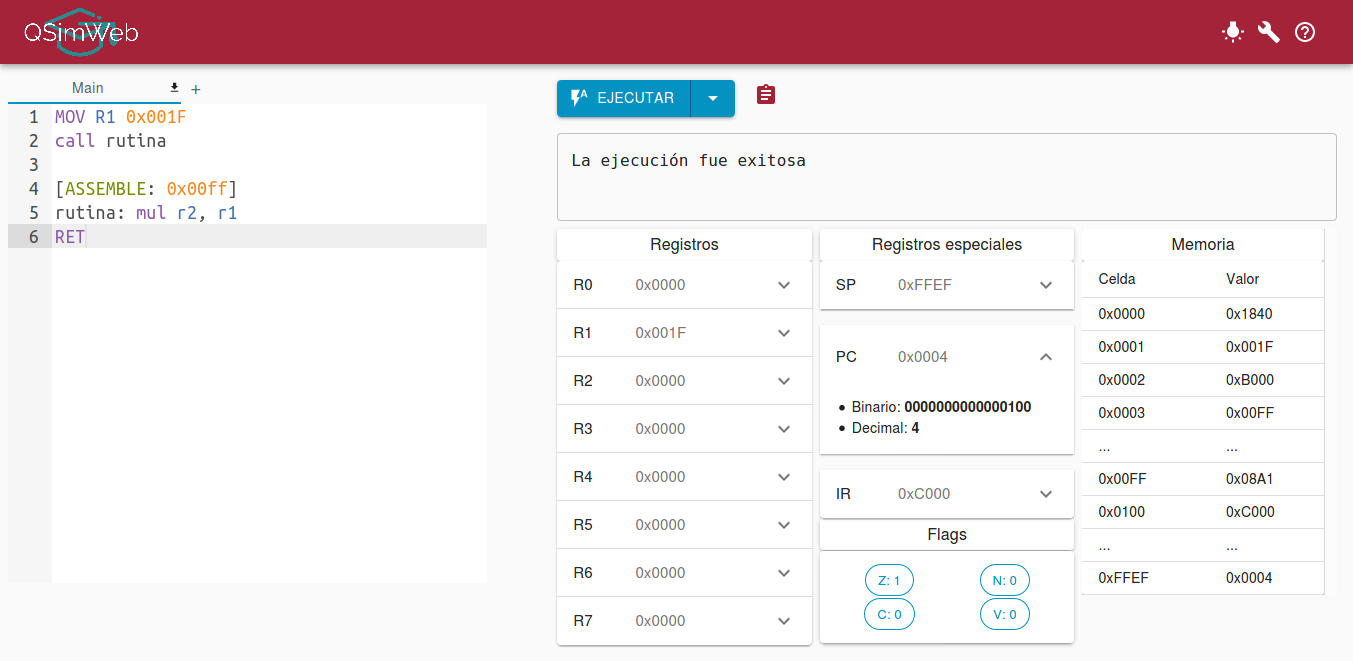
\includegraphics[width=14cm]{figuras/app-completa-bb.png}
\end{center}

\section{Proceso de ejecución}
Una de las necesidades principales es poder ejecutar código Q. La ejecución de un programa se compone de los siguientes pasos:

Se escribe un código Q en el editor de texto y se presiona ejecutar. 
Luego se analiza sintacticamente el texto que representa al programa, esta tarea es realizada por el Parser. 
Si ocurre un error se mostrará en pantalla informando lo ocurrido. Si el parseo pudo realizarse correctamente, se procede a 
traducir el resultado del parseo a instrucciones de la librería, esta tarea es realizada por el Translator.
Luego se procede a ensamblar y ejecutar el programa, ambas tareas son realizadas por Computer.
Si ocurre un error se mostrará en pantalla informando lo ocurrido. 
Si el programa finaliza, se mostrarán los resultados en pantalla.
\begin{figure}[H]
  \centering
  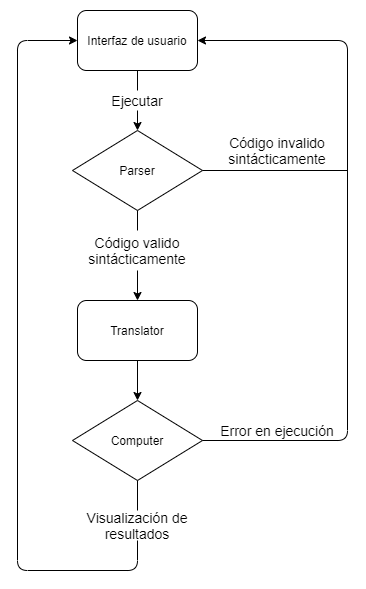
\includegraphics[width=10cm]{figuras/ejecucion_diagrama.png}
  \caption{Proceso de ejecución separado por componentes}
\end{figure}

Los detalles relacionados con la interfaz de usuario serán explicados en la sección que sigue a continuación.

Los detalles relacionados con la librería serán explicados en la sección ~\ref{qlib}


\section{Interfaz de usuario}

La interfaz cuenta con una pantalla inicial donde se pueden escribir y ejecutar programas Q, permitiendo visualizar los resultados de la ejecución. 
Además cuenta con una sección que permite configurar algunos aspectos de uso de la misma.

Se encarga de coordinar los pasos requeridos para ejecutar un programa utilizando la librería, es decir, parseo, traducción, ensamblado y ejecución del código. 

Las secciones nombradas anteriormente se describen a continuación:

\begin{center}
  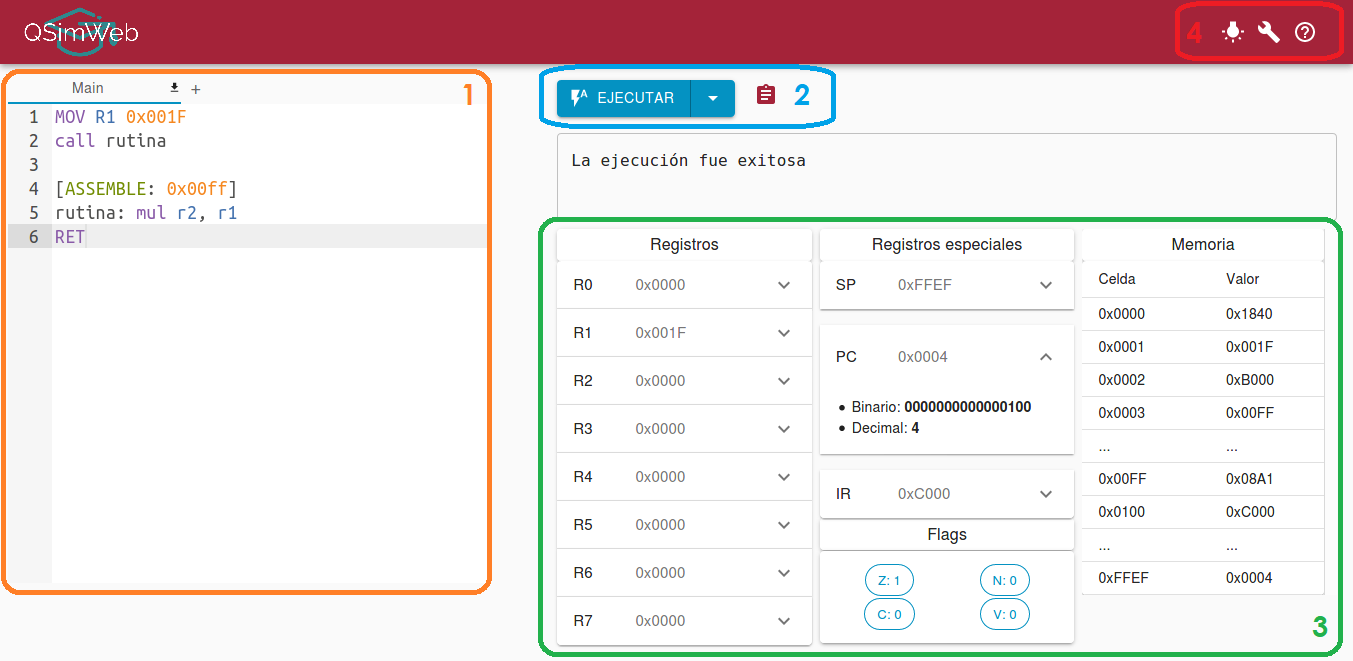
\includegraphics[width=14cm]{figuras/app-completa-dividida.png}
\end{center}

\subsection*{1. Editor}
Los programas se escriben sobre un editor de texto que cuenta con resaltado de sintaxis y errores. Estos programas pueden ser escritos tanto
en mayúsculas como en minúsculas. Cuando las instrucciones tienen más de un operando, estos pueden ser separados mediante uno o mas espacios o una coma.
El editor fue desarrollado utilizando la librería react-ace.

\begin{figure}[H]
  \centering
  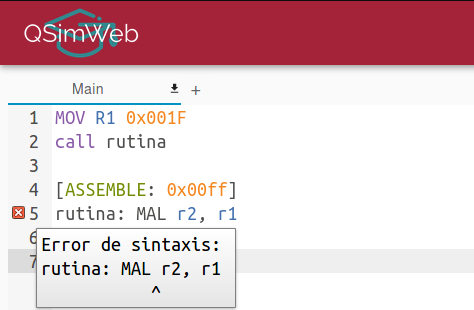
\includegraphics[width=10cm]{figuras/editor_errores.png}
  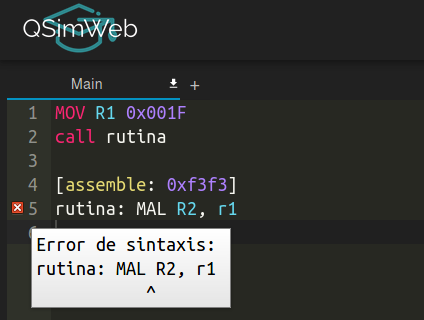
\includegraphics[width=10cm]{figuras/editor_errores_obscuro.png}
  \caption{Editor de texto con resaltado de sintaxis.}
  \label{fig:editor}
\end{figure}

Se permiten crear rutinas, ensamblandolas en celdas específicas utilizando [assemble: X], donde X es un inmediato representando la celda de memoria donde se ensamblará la rutina.
\begin{figure}[H]
  \centering
  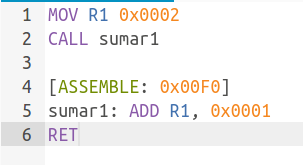
\includegraphics[scale=0.6]{./figuras/ASSEMBLE.png}
  \caption*{La meta instrucción ASSEMBLE permite indicar que la rutina sumar1 se ensamblará a partir de 0x00F0.}
  \label{fig:ASSEMBLE}
\end{figure}

\begin{figure}[H]
  La herramienta además permite la realización de comentarios que no afectarán la ejecución. Un comentario comienza con \# y termina al final de la línea.
  \begin{center}
    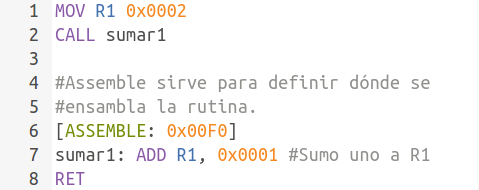
\includegraphics[scale=0.6]{./figuras/comentarios.png}
  \end{center}
  \label{fig:comentarios}
\end{figure}

\begin{samepage}
  Cuenta también con la posibilidad de dividir el código en distintas pestañas, importación de archivos .txt y descarga de los programas.
  
  \begin{center}
    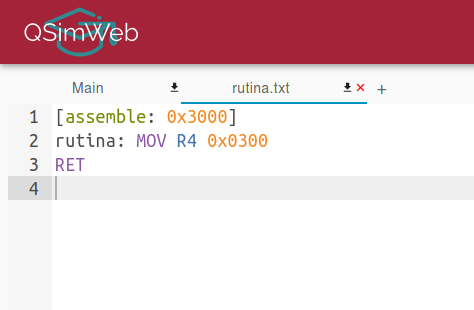
\includegraphics[width=10cm]{figuras/editor_tab.PNG}
  \end{center}
\end{samepage}

\subsection*{2. Botón de ejecución}
Cuando se quiere probar el código escrito, se debe ejecutar, haciendo click en el botón de ejecución.
La interfaz da la opción de ejecutar un programa de 3 modos distintos: Ejecución completa, Ejecución por instrucción y Ejecución por instrucción detallada. 
\begin{center}
  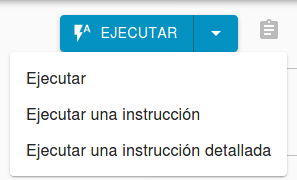
\includegraphics[width=7cm]{figuras/boton_ejecucion.png}
  \label{fig:boton-ejecucion}
\end{center}

El modo Ejecución completa realiza la ejecución de la totalidad de las instrucciones del programa mostrando, al final, los cambios en la sección de resultados. 

Ejecución por instrucción realiza la ejecución de una instrucción y muestra los cambios en la sección de resultados, al hacer click nuevamente, ejecutará la siguiente instrucción si existe. Si no existe se comenzará a ejecutar el programa nuevamente.

Para el modo de Ejecución por instrucción detallada, mostrará mensajes con las acciones producidas en cada paso de la ejecución. 

\begin{center}
  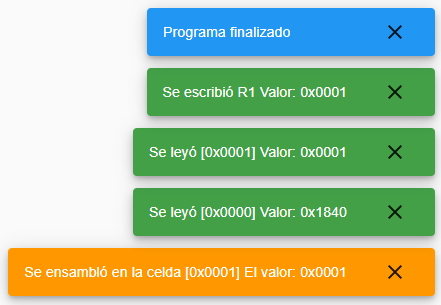
\includegraphics[width=8cm]{figuras/ejecucion_detallada.png}
\end{center}

En todos los modos de ejecución, dichas acciones quedan registradas y disponibles para su revisión:

\begin{center}
  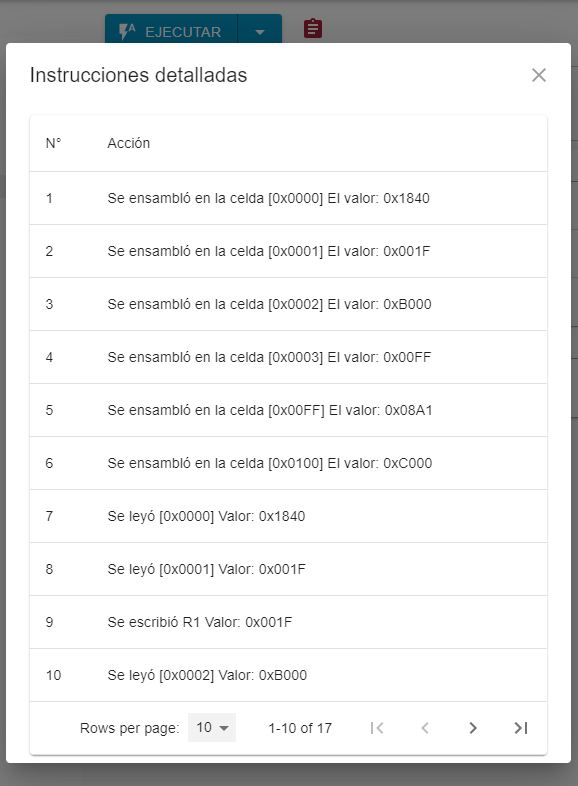
\includegraphics[width=9cm]{figuras/instrucciones_detalladas.PNG}
\end{center}

\subsection*{3. Resultados}
Una vez finalizada la ejecucion, con o sin errores, se actualizará la sección de resultados.

Los resultados se componen de los valores de registros, registros especiales, flags y memoria. Los valores de registros y registros especiales pueden ser
visualizados en hexadecimal, binario y decimal.
\begin{figure}[H]
  \centering
  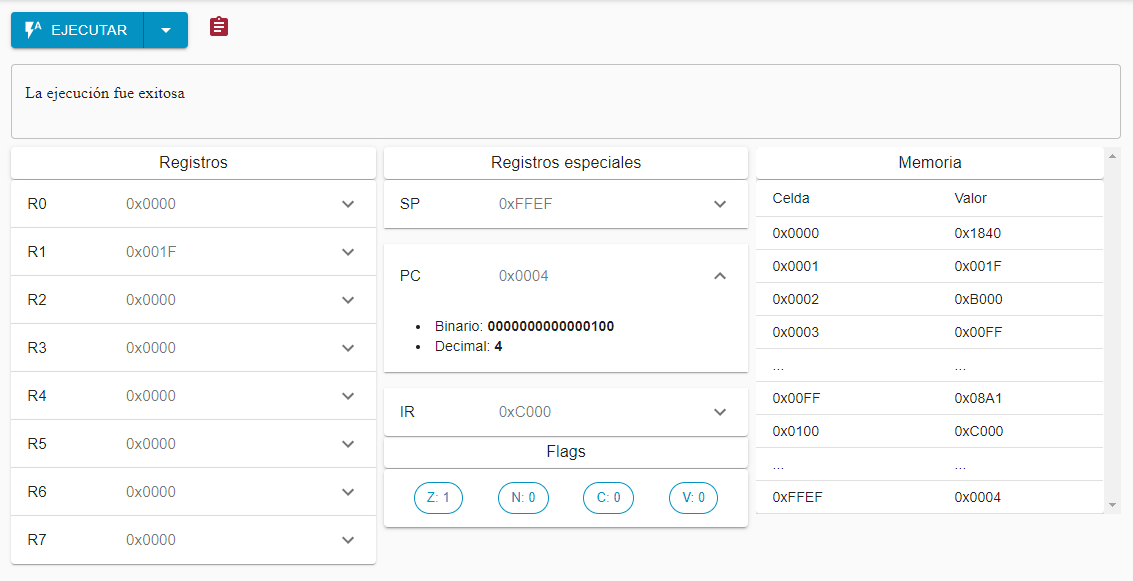
\includegraphics[width=14cm]{figuras/resultados.PNG}
  \caption{Resultados de la ejecución, separados en registros, registros especiales y memoria.}
  \label{fig:resultados}
\end{figure}

\begin{figure}[H]
  Cuando la memoria contiene celdas inicializadas que no son contiguas se resumen las celdas intermedias colocando "...".
  \begin{center}
    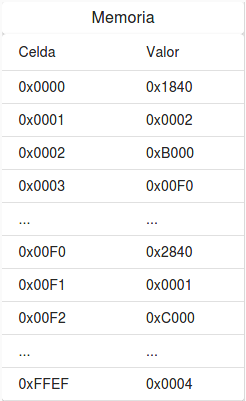
\includegraphics[scale=0.6]{./figuras/memoria_assemble.png}
  \end{center}
  \label{fig:memoria_assemble}
\end{figure}

Si durante la ejecución se produjo un error, este será mostrado en pantalla.
\begin{figure}[H]
  \centering
  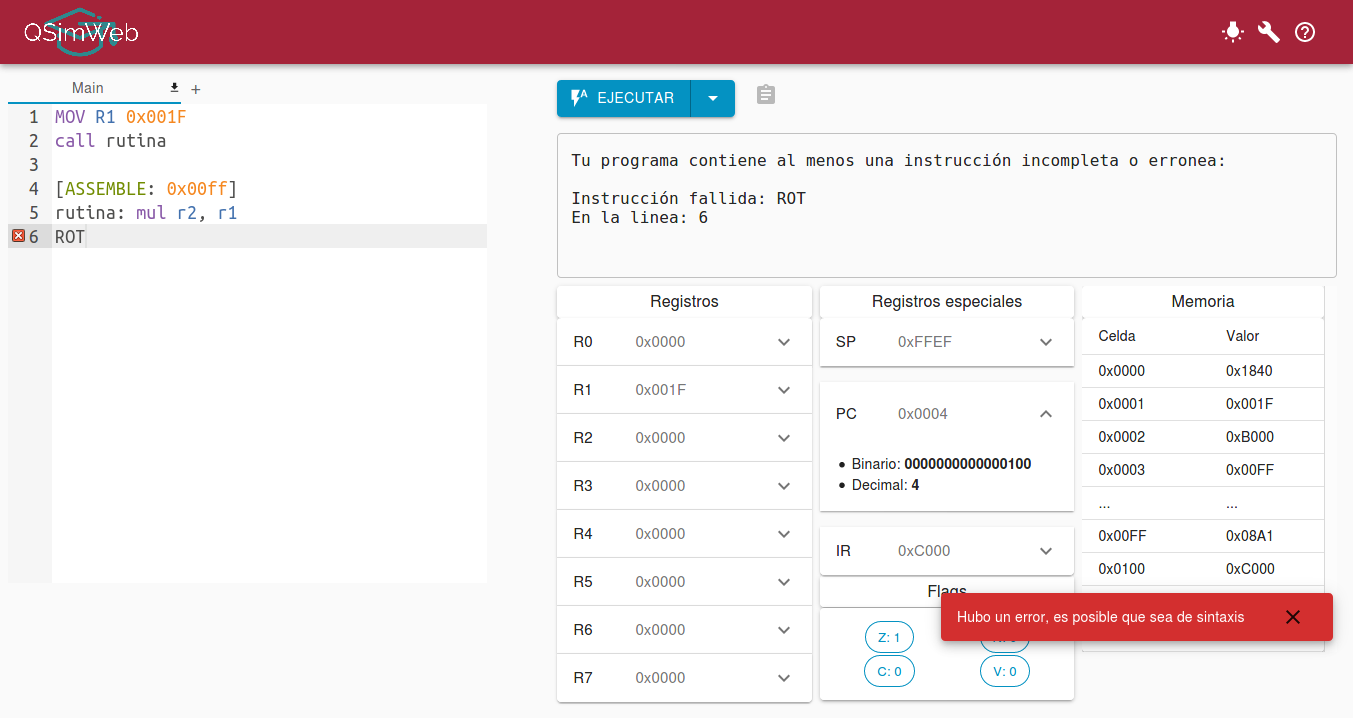
\includegraphics[width=14cm]{figuras/error.png}
  \caption{Error de sintaxis ocurrido al presionar ejecutar.}
  \label{fig:error}
\end{figure}

\subsection*{4. Configuraciones y ayuda}
La ventana principal cuenta además con un menú que permite configurar parametros de la ejecución.

\begin{center}
  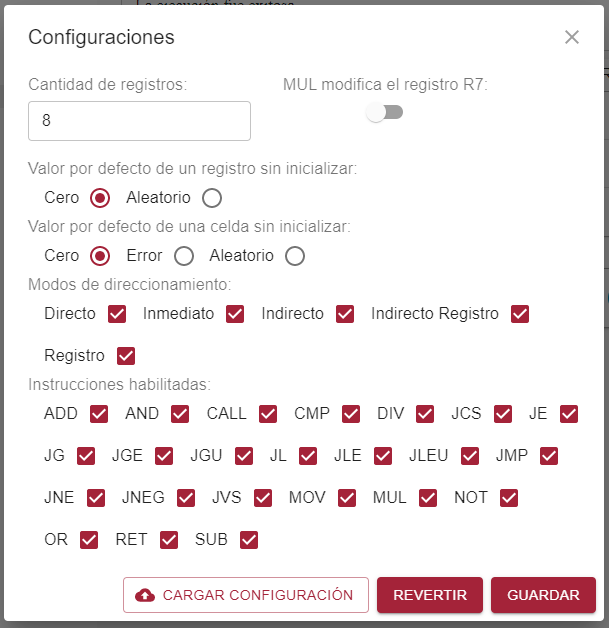
\includegraphics[width=8.7cm]{figuras/configuraciones.PNG}
\end{center}
En la configuración se permite cambiar la cantidad de registros, el comportamiento de MUL respecto al registro R7, los valores por defecto de las celdas de
memoria y registros, los modos de direccionamiento e instrucciones habilitadas. Es decir, todas las configuraciones que se especificarán en QConfig \referencia{subsec:qconfig}.
Además permite cargar un archivo de configuración para simplificar el armado de la misma.

Estas prefencias mencionadas se guardan en el navegador del usuario, permitiendo que no se pierdan al finalizar su uso.
Además se permite importar un archivo de configuración, donde se pueden especificar las configuraciones nombradas anteriormente. 

Se permite además ver un manual de uso.
\begin{center}
  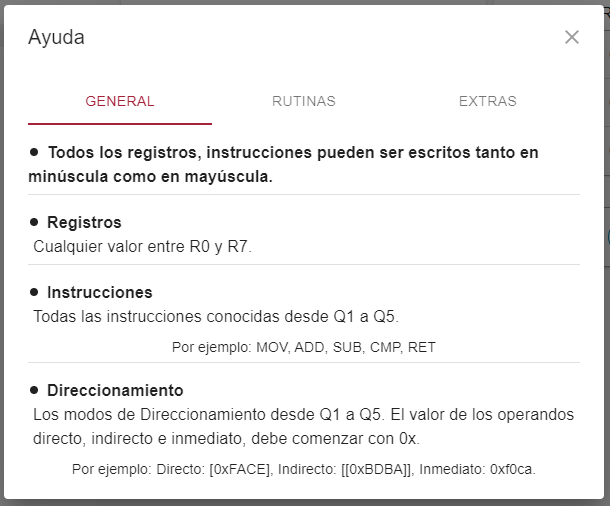
\includegraphics[width=8.7cm]{figuras/ayuda_general.PNG}
\end{center}

Existen los modos oscuro y claro, que facilitan el uso por parte de personas con daltonismo.
\begin{center}
  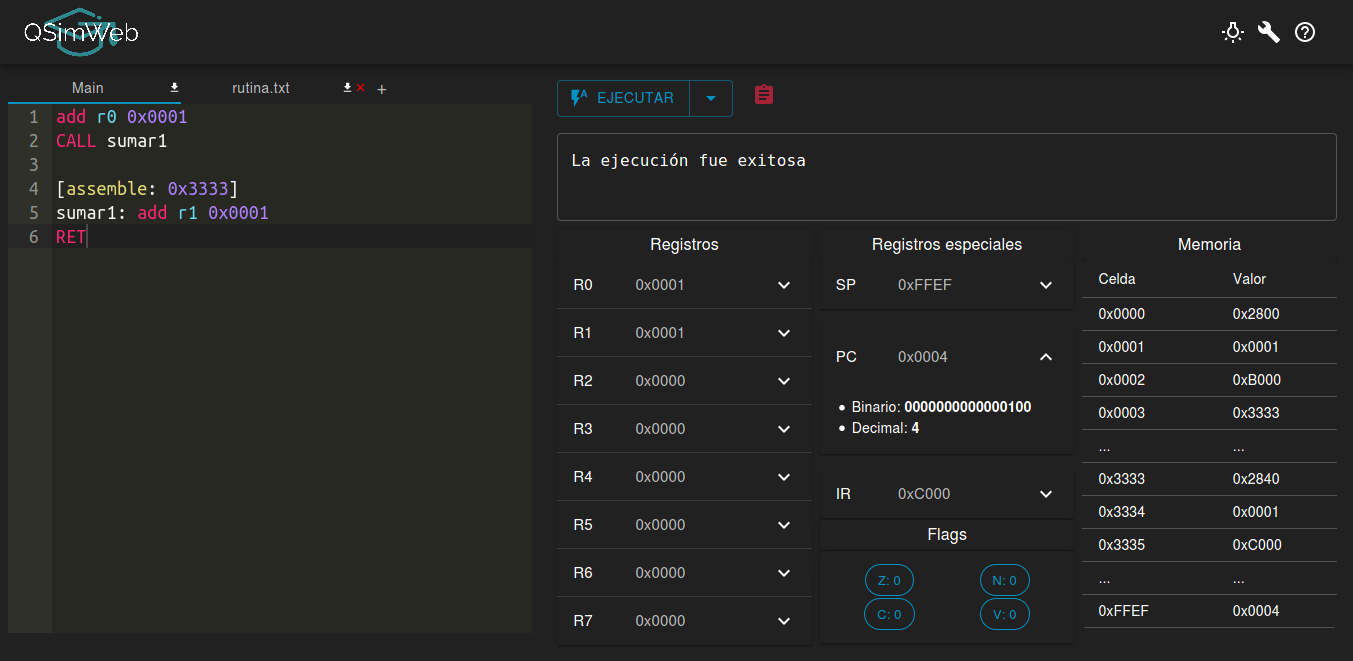
\includegraphics[width=14cm]{figuras/modo_obscuro.png}
\end{center}
\end{itemize}

\subsection{Accesibilidad}
\label{accesibilidad}

Una de las funcionalidades esperadas era brindar la posibilidad de la herramienta de ser usada con lectores de pantalla. En este sentido
se hicieron evaluaciones de accesibilidad utilizando herramientas estandarizadas y una prueba de campo con un estudiante no vidente de la tecnicatura.
Dichas evaluaciones permitieron hacer un diagnóstico de accesibilidad y posterior corrección de las fallas encontradas. Actualmente la 
herramienta contiene código para facilitar su uso, permitiendo que se pueda acceder a todas las funcionalidades de la misma.

Las mejoras realizadas hasta el momento fueron:
\begin{itemize}
  \item Nombrar correctamente el lenguaje de la aplicación ya que react pone por defecto el lenguaje en inglés.
  \item Agregar etiquetas a todos los botones.
  \item Agregar encabezados a la sección de resultados, para permitir su navegación y lectura.
  \item Corrección de autofoco en los modales.
  \item El contenido de las ventanas emergentes se lee automáticamente por el lector de pantalla.
\end{itemize}

\section{Librería}
\label{qlib}

La librería creada por este trabajo recibe el nombre de QLib. El objetivo de la creación de la librería es brindar una base de código que permita
la creación o modificación de herramientas para la enseñanza del lenguaje en el ecosistema de javascript, brindando así la posibilidad de ser
utilizada en navegadores web.
Además la existencia de una librería así, permite la creación de interfaces de usuario que extiendan a la entregada en este trabajo.

La misma esta compuesta por tres capas principales: Parser, Translator y Computer. Las funcionalidades que ofrece son:

\begin{itemize}
  \item Implementación del lenguaje Q: todas las instrucciones de Q, modos de direccionamiento, registros, flags, PC, SP, IR, MAR, MBR, etiquetas, pila están implementadas.
  \item Manejo de etiquetas: se proveen mecanismos para definir etiquetas, asociarlas a una dirección y utilizarlas en el ensamblado de programas.
  \item Manejo del ensamblado: métodos para pasar de un programa Q a la representación binaria de las instrucciones y viceversa.
  \item Ejecución completa, paso a paso y paso a paso detallada.
  \item Parseo del código Q.
  \item Capa de traducción entre el parseo y las instrucciones de la librería \referencia{subsec:translator}. 
  \item Opciones de configuración de la librería: modificar la cantidad de registros, valores por defecto de celdas y registros, modos de direccionamiento e instrucciones habilitadas en la ejecución.
  \item Exposición de valores del estado a lo largo de la ejecución.
  \item Exposición de acciones realizadas a lo largo de la ejecución.
\end{itemize}

Está diseñada utilizando el paradigma de programación orientada a objetos el cual define la existencia de clases y sus interacciones. 

\subsection{Parser}

El parser es la unidad encargada del analisis sintáctico para determinar si el programa es correcto de acuerdo a la gramática del lenguaje Q. 
Recibe como entrada una cadena de texto y devolverá objetos javascript en caso de ser la entrada sintacticamente válida o un error en caso 
contrario. Dicha salida será la entrada del Translator \referencia{subsec:translator}.

Para la definición de la gramática y su análsis sintáctico se utilizó la librería nearley.js, la cual provee una sintaxis para la definición de 
gramáticas basada en \textit{Extended Backus-Naur Form}. Los detalles de EBNF escapan al desarrollo de este trabajo por lo que es suficiente con 
pensar que este funciona como un metalenguaje, es decir, un lenguaje que permite la construcción de otros lenguajes. 

Para utilizar nearley.js se genera un archivo de gramática con la extensión .ne, donde se define la idea de instrucción, operando, tipos de 
instrucción y etiquetas. Luego, dicho archivo se compila a javascript utilizando la librería y esto permite el uso de la gramática en navegadores.

Una vez que la gramática está compilada, se utilizará la clase Parser provista por la librería para ingresar las instrucciones en forma de texto. 
Si son sintacticamente correctas, se devolverá un objeto preparado para traducirse a las instrucciones del lenguaje Q.

Este diseño que separa la etapa de parseo de la etapa de traducción a las clases del lenguaje permite la utilización de un parser distinto, siempre y cuando
su salida respete el formato esperado por el Translator.

\begin{figure}[H]
  \centering
  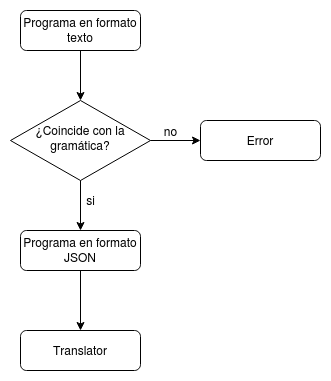
\includegraphics[width=7cm]{figuras/parser.png}
  \caption{Proceso de parseo del código.}
\end{figure}


\subsection{Translator}
\label{subsec:translator}
Como uno de los objetivos de QLib es permitir su utilización con distintos parsers, se provee una capa que actúe de interfaz entre los resultados 
brindados por el parser y las rutinas que utilizará la clase Computer para ejecutar el programa. 

En él se definen un conjunto de reglas que determinan cómo mapear las posibles entradas de formato JSON a instrucciones soportadas por QLib. Estas reglas 
se dividen en 3 grupos: \textit{reglas para instrucciones}, para \textit{tipos de instrucciones} y \textit{para operandos}.

\begin{figure}[H]
  \centering
  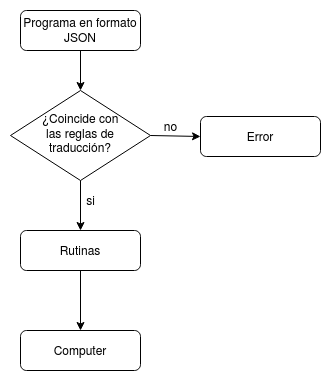
\includegraphics[width=7cm]{figuras/translator.png}
  \caption{Proceso de traducción del código.}
\end{figure}

Cuando se quiere traducir un programa, se realiza el siguiente proceso línea por línea:

En base a la línea que se está traduciendo, se busca una instrucción que coincida con el nombre de la misma en las \textit{reglas para 
instrucciones}. Una vez encontrada la instrucción, se busca el tipo de la instrucción en las \textit{reglas de tipos}. El tipo de la instrucción sirve para determinar
cómo se traducirán los operandos. Luego se obtienen los operandos de acuerdo al tipo de instrucción y el nombre del operando en las \textit{reglas para operandos}, 
obteniendo así, una instancia de operando de QLib. Con estas búsquedas realizadas se puede instanciar la instrucción de QLib y así armar las rutinas.
\subsection{Computer}

Esta capa tiene como funcionalidades principales el manejo del ensamblado y la ejecución. 

\subsubsection*{Ensamblado}
El ensamblado permite, utilizando las rutinas que genera el translator, obtener el código binario de las instrucciones para luego poder ejecutarlo. 
En el proceso de ensamblado intervienen principalmente 4 clases: Computer, Instruction, State y Memory. En esta etapa, la clase Computer se encarga 
de recibir las rutinas a ensamblar y delega en las instrucciones de cada rutina la obtención del código binario para entregarlo a la clase State.
State se encarga de guardar en memoria el código binario de cada una de las instrucciones utilizando la clase Memory.

\begin{figure}[H]
  \centering
  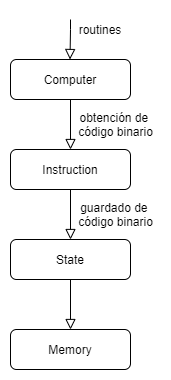
\includegraphics[width=3cm]{figuras/ensamblado.png}
  \caption{Proceso de ensamblado.}
\end{figure}

Como las instrucciones de una rutina pueden tener etiquetas o hacer uso de las mismas como operando, se definieron las clases Label y LabelReference 
para su manejo. Una rutina entonces, puede contener en su lista de instrucciones tanto elementos de tipo Instruction como de tipo Label.
El objetivo de la etapa de ensamblado es convertir las etiquetas en direcciones de memoria ya que las etiquetas son texto y este no puede ser
ensamblado en memoria. Para esto, el primer paso es calcular las direcciones de memoria donde se encuentren las definiciones de las etiquetas, es decir 
instancias de la clase Label. Luego, se deberán reemplazar los usos de esas etiquetas por operandos de tipo inmediato.

Para calcular las direcciones de memoria de las etiquetas se ven involucradas las clases Instruction y Label ya que son los elementos que puede
tener una rutina y el PC, que permite conocer la dirección de memoria actual. La clase Instruction, al solo representar instrucciones y no etiquetas, tiene la responsabilidad de avanzar el PC. Label en cambio,
tiene la responsabilidad de guardar el PC actual y su identificador en una lista de etiquetas y delegar en su instrucción el avance del PC.

\begin{figure}[H]
  \centering
  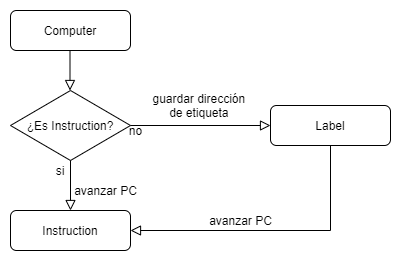
\includegraphics[width=8cm]{figuras/calculo-de-etiquetas.png}
  \caption{Cálculo de etiquetas.}
\end{figure}


\subsubsection*{Ejecución}

La etapa de ejecución se encarga de decodificar el código previamente ensamblado, traducirlo a instrucciones Q y ejecutarlas en orden.
De esta manera se da la noción de ejecución de un programa o rutina. Las instrucciones son decodificadas y ejecutadas de a una a la vez y esto permite
que el programa o rutina pueda mutar a lo largo de su ejecución. 

\begin{figure}[H]
  \centering
  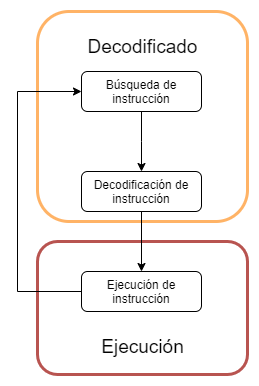
\includegraphics[width=4cm]{figuras/diagrama_ejecucion.png}
  \caption{Diagrama de ejecución.}
\end{figure}

Para ello, Computer lee la dirección de memoria indicada por el PC, cuyo contenido será decodificado. 
El decodificado del código máquina queda delegado en Instruction, ya que cada instrucción puede determinar si un código binario le corresponde y sabe
cómo decodificar sus operandos.
\begin{figure}[H]
  \centering
  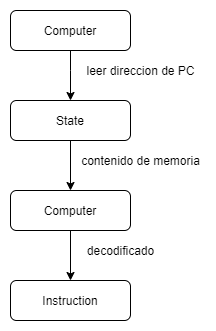
\includegraphics[width=5cm]{figuras/decodificado.png}
  \caption{Proceso de decodificado.}
\end{figure}

Una vez que la instrucción fue decodificada junto con sus operandos, se procede a ejecutarla. La ejecución de una instrucción recibe el estado actual y
lo modifica acorde a su efecto. Cada instrucción fue modelada con una clase, la cual conoce su efecto y lo aplica al ejecutarse. Este enfoque nos permite
agregar nuevas instrucciones facilmente siguiendo la interfaz brindada.

Estas modificaciones pueden incluir cambios en los flags, en el operando destino, en el PC o en la pila según la instrucción que se esté ejecutando.

Durante esta estapa pueden darse lecturas o escrituras de los operandos de origen y/o destino. Estos operandos pueden estar en modo inmediato, registro, directo,
indirecto o registro indirecto. Para conocer o modificar sus valores, los operandos dependen de los valores almacenados en el estado, quien guarda 
los valores de registros y conoce a la memoria. Es por ello que se definieron 5 clases para representar cada una de estas posibilidades, las cuales conocen
la forma de obtener valores del estado y guardarlos en él.

Como algunas instrucciones modifican los flags mientras que otras no lo hacen, esta tarea es delegada a cada instrucción, la cual conoce qué flags modifica
y cómo lo hace.

\begin{figure}[H]
  \centering
  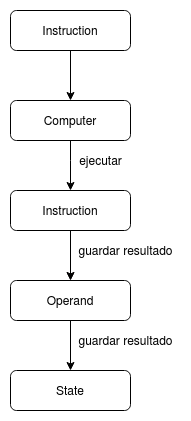
\includegraphics[width=4.5cm]{figuras/ejecucion_grafico.png}
  \caption{Proceso de ejecución.}
\end{figure}

\subsubsection*{La ejecución desde una mirada educativa}
En la definición de Q no existe la diferenciación de programa y rutina, como así tampoco la idea de finalización de ejecución. La computadora
está constantemente ejecucutando alguna instrucción, ya sea una instrucción con efecto o sin efecto.

Dado que QLib es una librería que simula una arquitectura de computadoras enfocada en la enseñanza, permite la creación de programas y rutinas. 
Estos se diferencian entre sí, porque los programas no finalizan con una instrucción RET mientras que las rutinas si. 

En la arquitectura Q no existe la idea de finalización de ejecución. Esto puede ser confuso para los/las estudiantes, ya que se esperaría que el programa tenga un inicio y 
un resultado final. Es por eso que consideramos que la librería debía proveer un método para identificar que la ejecución finalizó. 

Para ello, analizamos las siguientes condiciones: 

Al iniciar una ejecución las celdas que no hayan sido escritas, no tendrán valor. Por lo tanto el PC eventualmente llegará a una celda no incializada, esto puede darse por dos 
razones:
\begin{itemize}
  \item Un salto o una llamada a rutina en una celda vacía.
  \item Incremento orgánico del PC. Se considera que el PC se incrementó organicamente cuando su incremento no es causado por un offset o por una asignación directa.
\end{itemize}

Analizando dichas razones: 
\begin{itemize}
  \item Si se llega a una celda no inicializada mediante un salto o una llamada a rutina, asumimos que es un error de programación. Por ejemplo:
  \begin{center}
    MOV R1 R2 \\
    JMP 0x0fff \\
    \begin{footnotesize}
      En este caso se salta a la celda 0x0fff que no fue previamente inicializada.
    \end{footnotesize}
  \end{center}

  \begin{center}
    MOV R3 R0 \\
    CALL 0xAFFF \\
    \begin{footnotesize}
      En este caso se llama a la rutina ensamblada en la celda 0xAFFF que no fue previamente inicializada.
    \end{footnotesize}
  \end{center}

  \item Si se llega a una celda no inicializada mediante un incremento orgánico del PC pueden darse dos casos:
  
  La pila no está vacía, por lo tanto asumimos un error de programación. Posiblemente por el olvido de un RET.
  \begin{center}
    MOV R3 R0 \\
    CALL rutina \\
    MOV R0 R1 \\
  \end{center}
  \begin{center}
    [ASSEMBLE: 0x00ff] \\
    rutina: MOV R2 R3
  \end{center}
  
  La pila está vacía, puede haber dos razones:

  La etapa de ejecución no es \textit{FETCH} \footnote{FETCH es la etapa de la ejecución donde se busca en memoria la próxima instrucción a ejecutar.}. 
  \begin{center}
    MOV R3 [R0] \\
    \begin{footnotesize}
      En este caso, se lee el indirecto registro R0, pero la celda a la que apunta R0 no fue inicializada. Si bien esto no es un error, el resultado puede ser inesperado.
    \end{footnotesize}
  \end{center}
    
  La etapa de ejecución es FETCH, por lo tanto el programa finalizó.
  \begin{center}
    MOV R3 R0 \\
    CALL rutina \\
    MOV R0 R1 \\
  \end{center}
  \begin{center}
    [ASSEMBLE: 0x00ff] \\
    rutina: MOV R2 R3 \\
    RET
  \end{center}
\end{itemize}

\begin{samepage}
  Concluyendo, se asume la finalización de la ejecución cuando:
  \begin{itemize}
    \item La celda leída está no inicializada.
    \item El PC no fue modificado mediante un salto o una llamada a rutina.
    \item La pila se encuentra vacía.
    \item La etapa de ejecución es FETCH.
  \end{itemize}
\end{samepage}

\begin{figure}[H]
  \centering
  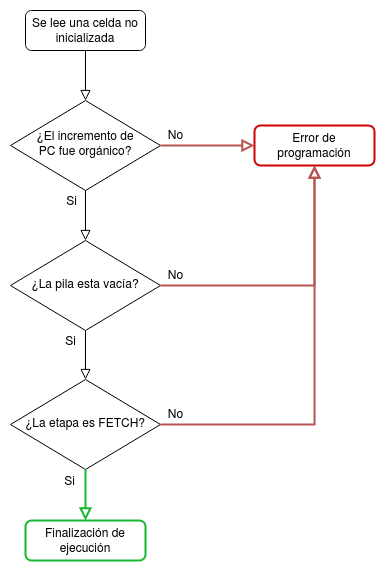
\includegraphics[width=7cm]{figuras/condicion_finalizacion.png}
  \caption{Condiciones de finalización.}
\end{figure}
\label{subsec:condfin}

Antes de definir una condición de finalización, tuvimos en cuenta la posibilidad de agregar una instrucción de fin, donde por ejemplo,
el usuario podría hacer uso de esta para definir cuándo o dónde el programa terminaría su ejecución.

Ejemplo de programa con instrucción de fin:
\begin{center}
  MOV R3 R0 \\
  ADD R0 R1 \\
  FIN \\
\end{center}

Con esta instrucción ya no sería necesario identificar una condición de finalización.

Optamos por definir una condición de finalización ya que esta facilita el entendimiento de un alumno o alumna de cuál es el resultado del 
programa que esté ejecutando abstrayendo la idea de que la computadora nunca deja de ejecutar. Por otro lado se evita agregar una instrucción que no 
se encuentra en Q.


\subsubsection*{QConfig}
\label{subsec:qconfig}
Existen distintos aspectos en QSim Web que pueden ser configurados con el objetivo de lograr que la herramienta tenga un enfoque más educativo y a su vez, 
para poder crear subconjuntos del lenguaje. QConfig es la clase encargada de guardar y modificar la configuración elegida. Existen las siguientes 
configuraciones:

\begin{itemize}
  \item Cantidad de registros: Permite modificar la cantidad de registros entre 1 y 8 (R0-R7). Si se intenta usar un registro deshabilitado, la 
  herramienta arrojará un error especificando lo sucedido.
  \item Comportamiento de la instrucción MUL: Permite elegir si se quiere que los 16 bits más significativos de una multiplicación se guarden en R7 o no.
  Esto es interesante ya que al principio resulta difícil de entender por los alumnos y que esté habilitado agregaría una complejidad esencial no 
  buscada en los comienzos de la materia.
  \item Valor por defecto en celdas: Permite elegir si el valor por defecto de una celda será cero; un error, si se intenta acceder al valor de una 
  celda no inicializada la herramienta lanzará una excepción; aleatorio, todas las celdas de memoria comenzarán con un valor aleatorio, 
  ayudando así a simular que la memoria siempre puede contener valores inesperados.
  \item Valor por defecto en registros: Permite elegir si el valor por defecto de un registro será cero o aleatorio.
  \item Modos de direccionamiento: Permite elegir qué modos de direccionamiento estarán habilitados en la ejecución. Si se intenta usar un modo de direccionamiento 
  deshabilitado, la herramienta lanzará una excepción indicando lo sucedido. 
  \item Instrucciones: Permite elegir qué instrucciones estarán habilitadas en la ejecución. Si se intenta usar una instrucción 
  deshabilitada, la herramienta lanzará una excepción indicando lo sucedido. 
\end{itemize}

Por ejemplo, si solo se requiere de Q1, basta con habilitar únicamente las instrucciones MOV, MUL, ADD, SUB y DIV y los modos de direccionamiento Inmediato y Registro.
\include{accesibilidad}
\part{Devoluciones de estudiantes}
\label{devoluciones}
Como parte del trabajo incluía una prueba de uso por estudiantes, se decidió compartir la herramienta en las comisiones de Organización de Computadoras
del segundo cuatrimestre del 2020.
Al finalizar la cursada fue enviada una encuesta para conocer las opiniones de los y las estudiantes acerca de la herramienta para poder saber qué tan útil resultó la herramienta y conocer ideas de posibles mejoras.

Los gráficos de los resultados obtenidos en la encuesta se pueden ver a continuación.
\begin{figure}[H]
  \centering
  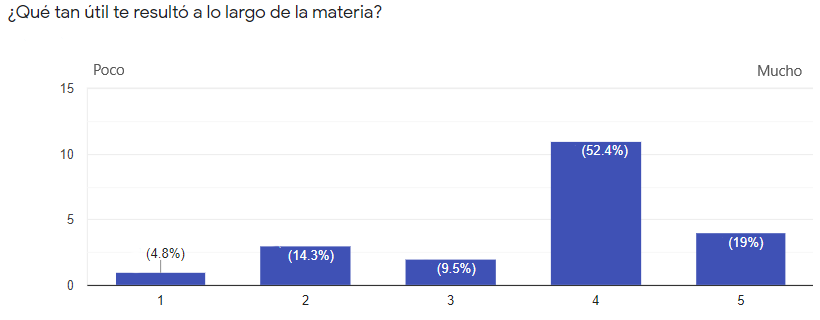
\includegraphics[width=16cm]{figuras/01_encuesta_que_tan_util.png}
\end{figure}

\begin{figure}[H]
  \centering
  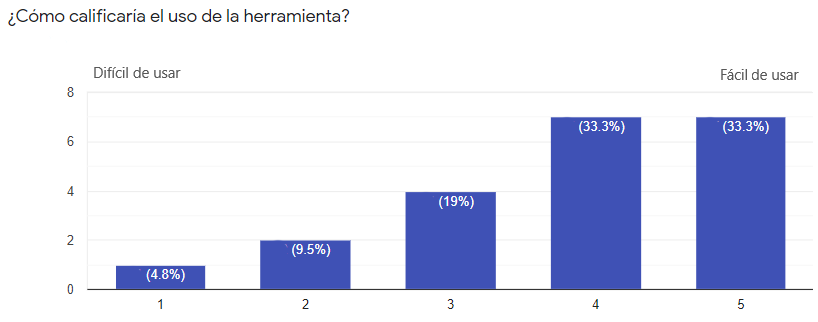
\includegraphics[width=16cm]{figuras/02_encuesta_uso.png}
\end{figure}

\begin{figure}[H]
  \centering
  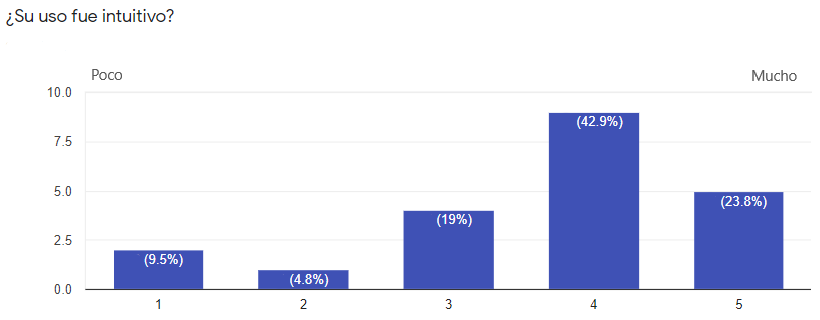
\includegraphics[width=16cm]{figuras/03_encuesta_uso_intuitivo.png}
\end{figure}

\begin{figure}[H]
  \centering
  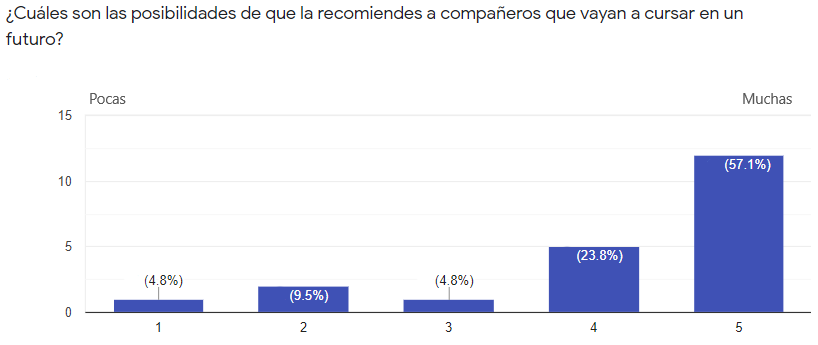
\includegraphics[width=16cm]{figuras/04_encuesta_posibilidad_recomendar.png}
\end{figure}

A pesar de que al comienzo del semestre los alumnos usaron una versión incompleta de QSim Web se puede observar, dado los resultados obtenidos, 
que la herramienta cumplió con su cometido, les fue útil, fácil de usar e intuitiva.

\begin{figure}[H]
  \centering
  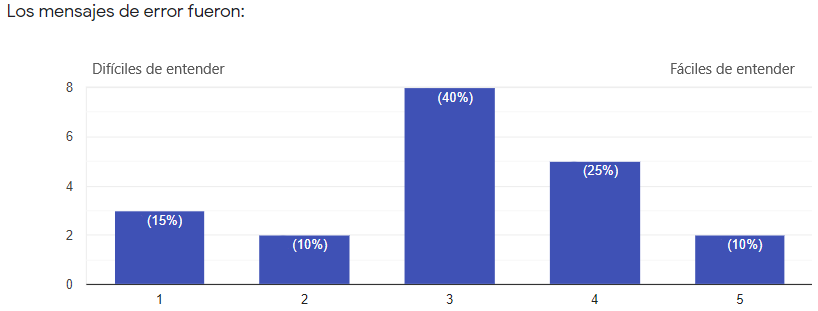
\includegraphics[width=16cm]{figuras/05_encuesta_mensajes_error.png}
\end{figure}
Aquí podemos observar, más allá de que el resultado no fue negativo, que los mensajes de error no fueron suficientemente declarativos.

\begin{figure}[H]
  \centering
  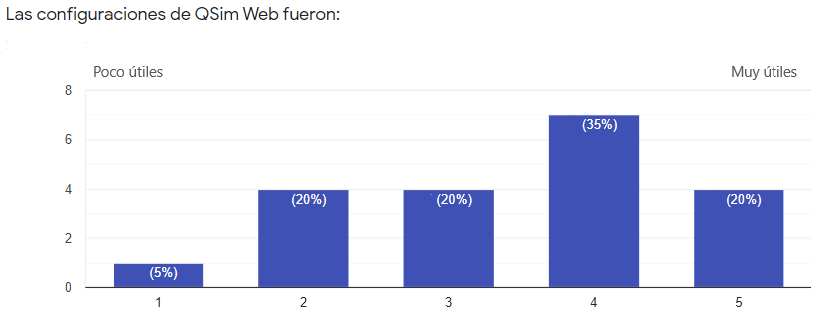
\includegraphics[width=16cm]{figuras/06_encuesta_configuracion.png}
\end{figure}
La configurabilidad de la herramienta nos parece un punto fuerte, pero al estar la mayoría de las funcionalidades habilitadas por defecto, esperábamos que aquí el gráfico tienda a “Poco útiles”. Nos sorprende positivamente que haya sido de utilidad.

\begin{figure}[H]
  \centering
  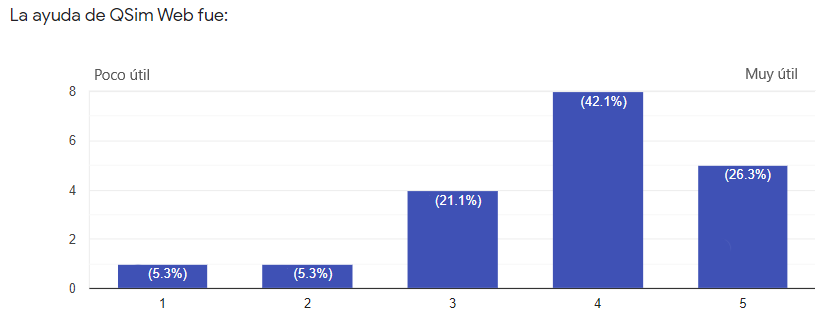
\includegraphics[width=16cm]{figuras/07_encuesta_ayuda.png}
\end{figure}

Además les hemos hecho preguntas donde se podían expresar de forma escrita. 
Estas preguntas apuntaban a conocer su opinión acerca de posibles mejoras de la herramienta, nuevas funcionalidades, funcionalidades que más gustaron y mejoras en la visualización
de resultados.
En general las respuestas fueron positivas y pudimos sacar varias conclusiones e ideas de nuevas funcionalidades para realizar a futuro, como se listarán a continuación.
Muchos comentarios no fueron realizados sobre la última versión de la herramienta, ya que la misma crecía con el pasar del cuatrimestre, y algunas de las funcionalidades pedidas
ya se encontraban implementadas.

Las nuevas funcionalidades son:
\begin{itemize}
  \item Mejorar la sección de ayuda.
  \item Mejorar descripción de errores de sintaxis.
  \item Mejorar resaltado de sintaxis.
  \item Visualización de resultados en Ca2.
  \item Dar la posibilidad de ejecutar instrucciones paso a paso automaticamente con un tiempo de diferencia entre cada una.
  \item Poder detener la ejecución.
  \item Resaltado de la linea de código que se está ejecutando.
  \item Cuando se detecta un error de sintaxis, además de marcarlo dar una posible solución.
  \item Poder modificar valores de registros, memoria y flags mientras se está ejecutando un programa.
\end{itemize}
\part{Conclusiones}
\label{parte_conclusiones}
El resultado de este trabajo es un simulador de la arquitectura Q que corre en un navegador y que puede ser usado por los y las estudiantes en 
el contexto de la materia Organización de Computadoras; permitiéndoles probar los programas que escriben, sin tener que simularlos en papel.
Además, fomentó la curiosidad, ya que realizaron programas por fuera de las prácticas y pusieron a prueba sus conocimientos. 

Desde el desarrollo de la herramienta notamos un aprendizaje en términos didácticos ya que habitualmente el software que realizamos en 
industria no es apuntado a la enseñanza. Sabemos que queda mucho por mejorar en este aspecto pero quienes hicimos este trabajo tenemos 
la intención de continuarlo para poder dar mejores funcionalidades tanto a estudiantes como a docentes.

Uno de los desafíos era la construcción de la idea de lenguaje, mediante el uso de gramáticas y parseo, aprendimos lo necesario para poder
completar el trabajo y seguramente sigamos aprendiendo a lo largo de la licenciatura.

Construimos una librería pensando en evitar siempre el acoplamiento a nuestra interfaz de usuario e incluso a nuestro parser, creemos que 
puede ser realmente el puntapie inicial para que otros/as estudiantes de la carrera puedan intervenir y mejorar el trabajo realizado.

\section{Trabajos futuros}
Encontramos durante el desarrollo algunas ideas que pueden incluirse a futuro:
\begin{itemize}
  \item Manejo de instrucciones I/O. Actualmente la arquitectura Q no define estas instrucciones pero podría ser una extensión que aporte
  interactividad a los programas.
  \item Permitir arquitecturas de computadoras distintas a Q, por ejemplo, poder variar el tamaño del bus de datos o direcciones.
  \item Incluir algún método de revisión docente, como por ejemplo deep link o envío de mails.
  \item Instrucción NOOP, para poder terminar programas sin necesariamente realizar una acción como última instrucción.
  \item Permitir la inicialización de registros y memoria antes de la ejecución.
  \item Mejorar el manejo de errores para mostrar mensajes más descriptivos.
\end{itemize}

\begin{thebibliography}{40}
\bibitem{Pattis} Richard E. Pattis, \textit{EBNF: A Notation to Describe Syntax}, University of California, Irvine.
\bibitem{Nearley} Nearley, \textit{How to grammar good}, \verb0https://nearley.js.org/docs/how-to-grammar-good
\bibitem{QSpec} \textit{Especificación - Q}, \verb0http://orga.blog.unq.edu.ar/wp-content/uploads/sites/5/2015/08/Especificacion-Q.pdf

%\bibitem{Enguix} A. Enguix,1984,  \textit{Clima y Mareas en el Río de la Plata (Wind \& Tide Pilot Book)}, Edición del autor.




\end{thebibliography}


\label{LastPage}
\end{document}
